 \chapter{Requirements and Analysis}

With the introduction to Manta Flow platform covered, we now have enough information required to understand and analyze the problem of embedded code analysis in its context. In this chapter we will analyze multiple technologies that support embedded code and formulate our requirements for the solution. Then we analyze how to integrate embedded code analysis into scanners. %% TODO rewrite after the chapter is finished

\section{Purpose of embedded code analysis}

We have already briefly explained what embedded code is and why it makes sense to analyze it in Manta Flow. Let us present an example that will support this explanation. It can help us build a better understanding of the motivation and illustrate some of the challenges that we need to overcome.
\par
This example is based on a real customer inquiry. A company has decided to move a part of their systems from self-hosted solution to a cloud-based solution. The migrated system cleans, pre-processes and combines data from multiple sources to create a high-quality data source for business analyses. They decided to use AWS (Amazon Web Services) as their cloud service provider. The new pipeline uses Amazon S3, Amazon Redshift and AWS Glue. Amazon S3 is a cloud object storage which is often used to store files used by other services. Amazon Redshift is a data warehousing service based on PostgreSQL database and optimized for scalability and big data processing. AWS Glue is an ETL tool which we have already introduced and will work with later in the thesis. The transformation jobs in AWS Glue are written in Python. The pipeline roughly follows these steps~(shown in figure~\ref{fig:pipelineExample}):
\begin{enumerate}
    \item Files containing raw unprocessed data are uploaded to Amazon S3.
    \item An AWS Glue job is executed which reads these files and normalizes the data - fills empty values, normalizes column names, etc. and stores it in a common data format under curated files on Amazon S3.
    \item Other AWS Glue jobs can be executed which read one or several curated files, combine the data and store it in a table in Amazon Redshift.
    \item Amazon Redshift is the final destination of this data pipeline. It is then used as a data source for visualisations and analytics.
\end{enumerate}

\begin{figure}[ht]\centering
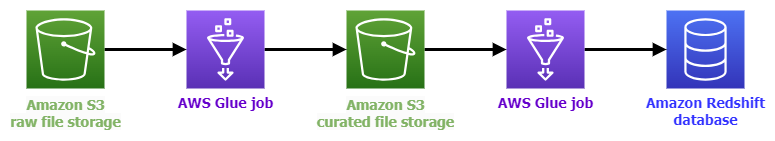
\includegraphics[width=1.0\textwidth]{img/pipeline_example.png}
\caption{A diagram of data flows in the pipeline}
\label{fig:pipelineExample}
\end{figure}

\par
Projects of this magnitude may take several months to complete, involve tens of employees who spend hundreds to thousands of man-days working on it. At this scale, it is important to keep a good overview on the progress to complete the project successfully. The customer has previously used Manta Flow to analyze different systems and would like to use it on this project as well. They would like to use it initially to watch the migration process and ensure that the new pipeline behaves correctly and no processes have been missed. After the project is over, they would like to continue using it to help with maintenance and problem resolution. The final dataset is a source for important financial and customer behavior analyses which directly impact many business decisions, so it is critical that the data is assembled correctly and data lineage visualization can help in that effort.
\par
How can data lineage analysis of embedded code help the customer? The pipeline consists of two data storage technologies, Amazon S3 and Amazon Redshift. They are only locations where data is stored. In order to find out how, for example, values in column \textit{average\_price} in table \textit{Sales} are computed, we must look into one of the AWS Glue jobs. An AWS Glue job runs a Python or Scala script on Apache Spark engine, which is a popular engine for large-scale data analytics. Therefore to provide the data lineage graph, we must run data flow analysis of the job's embedded code. When the analysis is successful, to find out how a value is computed we simply need to click on it in the visualized graph and follow the lineage. Without it we would have to locate the job manually, which might not be easy among 10s or 100s of them.

%%%%%% TODO
% 1 vziat requirements a rozpisat ich ako poziadavky zo strany Manty, zanalyzovat a vysvetlit ich
% 2 rozsirit analyzu technologii, pridat nejake priklady. 
% 3 Nasleduje analyza, ze to bude nejaka service atd, kde priblizime, ako funguje query service a porovnanie, co je stejne, co je odlisne a co by slo vyuzit
% Na konci kapitoly musi byt jasne, co ideme robit

\section{Requirements from Manta}

As this work has been assigned by and developed in cooperation with Manta Tools company which develops Manta Flow, they have set certain requirements that the final solution should fulfill. In this section we will first, state a requirement and then we will follow-up with a discussion about its motivation and implications.

\subsection{Functional requirements}

These requirements define what the solution nedds to and needs not to do.

\subsubsection{Embedded code analysis}

\textit{Provided a code script (string/file, not important implementation detail) and configuration, the service analyzes the script and delivers lineage graph for that script}. This requirement is pretty straight-forward, it describes what is to be delivered.
\par
Firstly, we shall discuss why a service is required. \textit{Service} is a wide term and its concrete meaning depends on the context. There is already \textit{Dataflow Query Service} in Manta Flow which handles analysis of embedded database queries and scripts. In its core it is a Java bean (a class that encapsulates one or more objects into a single standardized object) which uses specific parts of database scanners to process the queries. It is called a service, because it is a reusable component (a bean) that can be used by any scanner and it provides its services through a standardized interface with a specific input and output. The solution described in this work, Embedded Code Service, is in many ways similar to Dataflow Query Service so it is expected to be used in a similar way.
\par
The service shall accept embedded code as one of its inputs. That is different from how scanners in Manta Flow usually work, because they collect their inputs themselves. It shall also accept configuration. What will it be used for? Scanners in Manta Flow have many configurable properties which influence their execution, users may modify them in \textit{Manta Admin UI}. It must be possible to configure how embedded code is analyzed as well. Additionally, from the description of embedded code we know that it is executed in the environment provided by the data technology. This environment can differ from standard runtime environment, so any differences, e.g. environment variables, pre-included libraries, need to be passed to the service in some way - in the configuration.
\par
The last part of this requirement describes that the service shall perform data flow analysis of the input and provide the data lineage graph on the output for further processing. Contrary to the standard scanner workflow, the Manta graph is not uploaded to \textit{Manta Flow Server}, but returned as return value.

\subsubsection{Graph merging}

\textit{The service can merge the lineage graph with the lineage graph of parent data technology when provided a node to be merged with}. This requirement extends the previous one and describes what is to be done with the output.
\par
Each scanner produces one Manta graph for one input. When it uses a service to process a part of the input, which creates other graphs, they need to be merged. The merge operation is not a trivial process, so it shall be the responsibility of the service to implement it. The benefits are easy to see, no need to implement it each time the service is used across different scanners, which improves maintainability of the solution and also there is no need to understand it outside of the service. The developers may simply use the service interface to merge the results.

\subsubsection{Multi-purpose service}

\textit{The service can support multiple parent data technologies - technologies that support usage of user-defined embedded code}. This requirement states that the service is multi-purpose, so there is one such service available instead of there being many services for processing embedded code in each data technology.

\subsection{Qualitative (non-functional) requirements}

On top of the definition of functionality of the solution, there are also some requirements defining its qualities.

\begin{enumerate}
    \item The service should be optimized to handle tens to hundreds of scripts for a specific combination of technology-scanner in one analysis - the limitation should be the speed of the scanner, not speed of the service
    \item Extending supported technologies should be simple - adding a new technology should only include collecting its configuration in the technology scanner and implementing this configuration in embedded code service
    \item Maximizing code reuse - reuse the existing scanners and logic
    \item Minimizing code duplication - no logic should be written on more than one place
\end{enumerate}



%%----- SECTION -----%% An extended problem overview, analysis of supported/desired technologies that support embedded code.
\section{Embedded scripts in data technologies}
% Why we analyze scripts
Let us briefly 
Execution of embedded scripts is one of the essential features of many data technologies. It moves usability of the data technology to the next level as the users are able to define custom ways to modify and work with data. It brings more possibilities to automate data manipulation processes.
\par
Stored procedures and functions in databases are often used to simplify data manipulation processes. Often, it takes several SQL commands to achieve a desired change. Instead of having to remember the exact chain of commands, it is easier to call a procedure that implements it. For example, in figure~\ref{fig:storedProcedure} we can see a simple stored procedure that retrieves a list of Czech employees without the need to define the query. They are also beneficial when data processing is automated, the same procedure may be called repeatedly with different parameters to process different inputs. When analyzing data lineage in a database, these scripts contain most of the observable data flows, so analyzing them is the key objective.
\begin{figure}[ht]
\begin{lstlisting}[language=SQL] 
CREATE PROCEDURE czechEmployees AS
SELECT ID, FirstName, LastName
FROM Employee
WHERE CountryCode = 'CZ';
\end{lstlisting}
\caption{An example of SQL Server stored procedure}
\label{fig:storedProcedure}
\end{figure}
\par
ETL technologies often provide a standard tool box that contains different data source providers for reading and writing data and many commonly used transformations. A user may create their ETL pipeline just by connecting them in a graphical interface. However, the developers are not always able to cover all use-cases the users might need. They might want to connect to a recently released database or an already supported database, but which is secured in a non-standard way. They might want to filter or transform data based on value properties that cannot be easily expressed in SQL or in a way specific to their data. Furthermore, platforms such as AWS Glue may just provide a scalable, secure, serverless cloud environment for pipeline execution where the user is expected to provide the pipeline code (see figure~\ref{fig:embeddedScript}). In these cases, data lineage analysis of embedded scripts is necessary to capture an integral part of data flow, otherwise it may become fragmented, because a piece is missing. Sometimes it may even contain the entire data flow in the pipeline. While ETL tools are great for data processing, they are not always the best environment for code development. The main negatives from software development point of view are limited debugging, testability and version control support of embedded code. Embedded code is executed in a custom internal runtime environment of the data technology and its replica for development is not always available. For that reason there is also a demand for systems that can bridge this gap and verify the correctness of embedde scripts. One of the ways to check it is utilising data lineage analysis to verify that the data flow as expected.
\begin{figure}[ht]
\begin{lstlisting}[language=Python]
import sys
from awsglue.transforms import Join
from pyspark.context import SparkContext
from awsglue.context import GlueContext

glueContext = GlueContext(SparkContext.getOrCreate())

db_name = "main_db"
output_dir = "s3://glue-example/output/supply_chain"

# Create dynamic frames
products = glueContext.create_dynamic_frame.from_catalog(database=db_name, table_name="products_json")
purchases = glueContext.create_dynamic_frame.from_catalog(database=db_name, table_name="purchases_json")
suppliers = glueContext.create_dynamic_frame.from_catalog(database=db_name, table_name="suppliers_json")

# Keep the fields we need and rename some
products = products.drop_fields(['color', 'identification']).rename_field('name', 'product_name')

# Join the frames
result = Join.apply(Join.apply(products, purchases, 'id_product', 'product_id'), suppliers, 'supplier_id', 'id_supplier')

# Write out the frame into parquet file
glueContext.write_dynamic_frame.from_options(frame = result, connection_type = "s3", connection_options = {"path": output_dir}, format = "parquet")
\end{lstlisting}
\caption{An example of an embedded script in AWS Glue}
\label{fig:embeddedScript}
\end{figure}

\subsection{Embedded scripts in Manta Flow}

The main goal of this work is to enhance Manta Flow with the ability to process embedded scripts written in a programming language
Automated data flow analysis of embedded scripts in Manta Flow is not an easy task. Because the script is analyzed outside of the execution environment, it cannot be executed and the particular scanner has to perform static code analysis. Such algorithm not only has to be able to parse the code, but it also has to \textit{understand} it to be able to detect when and from where data is loaded or written to and track it as it is propagated and transformed. Take the code in figure~\ref{fig:sqlVariable} for example, the scanner has to \textit{understand} that a value in column \texttt{cust\_id} of \texttt{customers} table is assigned to the variable \texttt{@id}, remember this data flow and then correctly conclude that this value is written to the \texttt{customer\_id} column of the \texttt{orders} table. It is, of course, only one simple example of many, the problem gets more complicated when complex joins, user-defined functions which are defined outside a script, etc. get involved. The bottom-line is that it is desired to implement the analysis of one language's code in exactly one scanner so the complexity remains maintainable.

\begin{figure}[ht]
\begin{lstlisting}[language=SQL]
SELECT @id := cust_id FROM customers WHERE cust_id='customer name';
INSERT INTO orders (product_id, customer_id, quantity) VALUES (123, @id, 1);
\end{lstlisting}
\caption{Data propagation through a variable in MySQL}
\label{fig:sqlVariable}
\end{figure}

\par



Supporting the analysis of embedded scripts in Manta Flow is not always as simple as running the particular scanner with the code as its input. Each input is also tightly dependent on the environment where it is executed. Since the analysis of programming languages is so complex, we want to use the existing scanners as much as possible. However, original implementations of these scanners were developed to be able to process applications written in the particular programming language. They are designed to run in standalone scenarios and their configuration mostly defines where the application can be found. We need to modify these scanners so they can be reused by other independent data technology scanners in their scenarios in a meaningful way.
\par % how query service does it
A similar problem has been solved by Dataflow Query Service which allows other scanners to process database queries. These database queries need to be processed by a particular database scanner, because different databases use different SQL dialects and also because Query Service results are enriched with the mapping to the actual data sources that has been analyzed by that scanner, if possible. We will inspire by its design because it solves two similar problems: providing a partial lineage graph to be used in another lineage graph and executing the analysis of one scanner in the scope of another.
\par % how we shall do it
Our solution shall provide an embedded code service which can be integrated and used in other scanner scenarios. It shall provide an interface to configure the input and execute the analysis of the provided embedded code and it shall provide an interface to integrate the resulting lineage graph with the lineage graph of another data technology.

%%----- SECTION -----%%
\section{Source technology analysis}

Before we dive further into the analysis, we need to examine which source technologies, whether currently supported by Manta Flow or planned, support embedded code. This overview will give us a better understanding of the range of embedded code use-cases as well as help us in choosing a candidate for a proof-of-concept implementation.

\subsubsection{Hive}
Hive is a distributed data warehouse system that allows users to read, write and manage big volumes of data using SQL. Starting from version 0.13.0, it supports writing user-defined functions in Java which accept parameters and return a value. The function is implemented by a class that extends a Hive UDF base class. These base classes define methods that shall be implemented by the function and will be invoked in specific order on SQL query execution. This class is then supposed to be packaged in a JAR referenced by a URI from which it will be loaded into the environment~\cite{hive}.

\subsubsection{Microsoft SQL Server}
Microsoft SQL Server enables users to implement stored procedures, triggers, user-defined types, user-defined functions (scalar and table valued), and user-defined aggregate functions using any .NET Framework language, including Microsoft Visual Basic .NET and Microsoft Visual C\#. They can be implemented by arbitrary classes and methods as long as they are properly annotated. These annotations facilitate the lookup and binding between SQL Server and embedded code. Compiled code is distributed in DLL and loaded into environment using SQL syntax~\cite{mssql}.

\subsubsection{SQL Server Integration Services (SSIS)}
SSIS is a platform for data integration and transformation solutions. It provides graphical tools for building ETL workflows, but it is also possible to create custom objects programmatically in C\# or Visual Basic. These include tasks, connection managers, log providers, enumerators and data flow components. Implementations of custom objects are expected to extend one of the base classes provided by SSIS, to override required methods and to use proper attributes. These objects are then distributed as a compiled class library. This is a similar approach as that of MSSQL~\cite{ssis}.

\subsubsection{PostgreSQL}
By default, PostgreSQL supports functions written in C, but theoretically users may use any language, as long as it can be made compatible with C, e.g. C++. However, that is often difficult due to different calling conventions, so its safe to assume C language is used. The function definitions are supposed to use macros from \texttt{postgres.h} header file, but otherwise are common C functions. The code is compiled and dynamically loaded into the environment using SQL. There is currently no plan to support analyzing C language, so this data technology is mentioned only for completeness~\cite{postgresql}.

\subsubsection{Snowflake}
Snowflake Data Cloud is a cloud-based data storage and analytics service. It is common to use SQL to interact with data in Snowflake and embedded code is integrated in a similar way in the form of functions and stored procedures. Apart from SQL, these can be written in multiple programming languages - Java, Scala, JavaScript or Python. Each language used has (slightly) different capabilities and requirements. In case of JavaScript, it can be used to execute SQL statements and interact with the result to provide a return value. Java, Scala and Python scripts have to contain a function or a method with the first argument of type \texttt{Session} from Snowflake's Snowpark library. This argument will be populated by Snowflake when the procedure/function is invoked and is used for interaction with Snowflake platform~\cite{snowflake}.

\subsubsection{Databricks}
Databricks is a web-based data platform that combines data warehouses and data lakes with analytics build on Apache Spark and IPython-style notebooks. These notebooks are interactive computational environments. They consist of a sequential combination of cells which may contain rich text, embedded code, data visualization etc. Embedded code cells may be written in Python, Scala, SQL or R and it is possible to combine cells written in different languages in one notebook. During a notebook execution, cells written in the same language are executed in the same environment and may interact with other language environments using shared context of Apache Spark~\cite{databricks}.

\subsubsection{AWS Glue}
AWS Glue is an ETL tool that supports interactive ETL pipeline creation and then generating code for Apache Spark in Python or Scala that executes the pipeline. This code can then be further modified. Compared to other data technologies, AWS Glue is built entirely on embedded code. That means that each ETL job is executed entirely by a single Python/Scala script as opposed to only parts of data operations in other data technologies~\cite{awsglueintro}. 

\subsubsection{Other data technologies}
Besides the data technologies already described, there are others that provide embedded code integration and are supported in Manta Flow. These follow similar principles as some that were already described before, so we will not cover them in detail. However, we list them below for completeness:
\begin{itemize}
    \item Talend supports extending the functionalities of a Talend Job using custom Java commands~\cite{talend}.
    \item Google BigQuery supports defining functions written in JavaScript~\cite{bigquery}.
    \item StreamSets allows creating custom StreamSets processors in Java~\cite{streamsets}.
    \item Informatica supports creating custom components with Java~\cite{informatica}.
    \item Azure Data Factory supports creating Custom activity with own data movement or transformation logic in C\# that can be added to a pipeline~\cite{adf}.
    \item SAS supports running Python statements within a SAS session~\cite{sas}. Additionally, there are multiple Python packages for interacting with SAS from Python.
\end{itemize}

\subsection{Embedded code usage philosophy}
Based on the description of embedded code usages, we can observe a few repeating patterns. These will help us design embedded code service.
\par
We can see that database systems use embedded code in the form of user-defined functions or stored procedures. They can then be invoked as a part of an SQL query or an SQL script. They often return a value and may receive arguments.
\par
Another common use-case is to define a custom transformation or a task in an ETL workflow. The details of this use-case vary more than those in database systems but in general they implement a specific interface which functions are invoked in a pre-determined order by the data technology.
\par
Next observation relies to the programming language being used. Most often we can see Java or Scala, .NET languages (mainly C\# or Visual Basic) and Python. Sometimes also JavaScript is used and there is one case of R and C, but we shall ignore them as there isn't currently a language scanner implemented in Manta Flow for them.
\par
In compiled static-typed languages (Java and C\#), it is common to tag the classes that shall be used as embedded code and require a rigid interface, either by extending a base class or using annotations. The code is distributed in compiled form and loaded dynamically. Interaction with the data technology is facilitated through an object that is provided as a method argument or a property of a base class.
\par
As Python is interpreted and not compiled, it is possible to inject the embedded code into a different code to create a new script. That allows use-cases where some code is executed before embedded code which defines some variables, functions, classes etc. The embedded code may then directly read these identifiers without having to declare them, which is used to provide interface for interacting with data technology. To successfully analyze such approach, it is important to understand and simulate these assignments.

%%----- SECTION -----%% Functional and qualitative requirements
